\documentclass{article}
\usepackage{CTEX}

%%%%%%%%%%%%%%%%%%%%%%%%%%%%%%%%%%%%%%%%%%%%%%%%%%%%%%%%%%%%%%%%%
\usepackage[a4paper]{geometry}
\geometry{left=3cm,right=3cm,top=3cm,bottom=3cm}
\linespread{1.5}
\usepackage{fancyhdr}

\usepackage{fontspec}
\defaultfontfeatures{Mapping=tex-text}
\usepackage{xunicode,xltxtra}
\usepackage[BoldFont,SlantFont,CJKnumber,CJKchecksingle]{xeCJK} \usepackage{CJKfntef}
\usepackage{bm} 
\usepackage{pifont}
\usepackage{color,xcolor}
\definecolor{GREEN}{RGB}{25,180,68}
\definecolor{YELLOW}{RGB}{255,255,224}
\definecolor{BLUE}{RGB}{65,105,225}
\definecolor{RED}{RGB}{139,0,0}
\definecolor{DRED}{RGB}{128,0,0}
\definecolor{GREY}{RGB}{128,128,128}

\usepackage{amsmath,amsfonts,amssymb}

\usepackage[americaninductors,europeanresistors]{circuitikz}
\usepackage{tikz}
\usetikzlibrary{positioning,arrows,shadows,shapes,calc,mindmap,trees,backgrounds}
\usepackage{graphicx}
\usepackage{subfigure} 
\usepackage{colortbl,dcolumn}  
\usepackage{multirow}
\usepackage{multicol}
\usepackage{booktabs}
\usepackage{fancyvrb}
\usepackage{listings}

\usepackage{titlesec}
\usepackage{etoolbox}
\makeatletter
\patchcmd{\ttlh@hang}{\parindent\z@}{\parindent\z@\leavevmode}{}{}
\patchcmd{\ttlh@hang}{\noindent}{}{}{}
\makeatother
\usepackage{mdwlist}
\usepackage{verbatim}
\usepackage{/Users/jinna/styles/zhfontcfg}
\usepackage{/Users/jinna/styles/visionouclistings}
\usepackage{/Users/jinna/styles/visionouccfg}
\setlength{\headheight}{15pt}
\fancyhf{}
\setCJKmainfont{Adobe Kaiti Std} 
\setCJKmonofont{Adobe Fangsong Std}
\makeatletter
\def\headrule{{\if@fancyplain\let\headrulewidth\plainheadrulewidth\fi%
\color{BLUE}
\hrule\@height 2.5pt \@width\headwidth\vskip1pt 
\hrule\@height 0.5pt\@width\headwidth              
\vskip-2\headrulewidth\vskip-1pt}        
\vspace{6mm}}                
\makeatother         

\graphicspath{{figures/}}
\tikzset{
    >=stealth',
    punkt/.style={
           rectangle,
           rounded corners,
           draw=black, very thick,
           text width=6.5em,
           minimum height=2em,
           text centered},
    pil/.style={
           ->,
           thick,
           shorten <=2pt,
           shorten >=2pt,},
    FlyZhyBall/.style={
      circle,
      minimum size=6mm,
      inner sep=0.5pt,
      ball color=red!50!blue,
      text=white,},
    FlyZhyRectangle/.style={
      rectangle,
      rounded corners,
      minimum size=6mm,
      ball color=red!50!blue,
      text=white,},
    zhyfly/.style={
      rectangle,
      rounded corners,
      minimum size=6mm,
      ball color=red!25!blue,
      text=white,},
    nrectangle/.style={
      rectangle,
      draw=#1!50,
      fill=#1!20,
      minimum size=5mm,
      inner sep=0.1pt,}
}

% code
\lstnewenvironment{VHDLcode}[1][]{%
  \lstset{
    basicstyle=\footnotesize\ttfamily\color{black},%
    columns=flexible,%
    framexleftmargin=.7mm,frame=shadowbox,%
    rulesepcolor=\color{blue},%
%    frame=single,%
    backgroundcolor=\color{yellow!20},%
    xleftmargin=1.2\fboxsep,%
    xrightmargin=.7\fboxsep,%
    numberstyle=\tiny\color{blue},%
    numberblanklines=false,numbersep=7pt,%
    language=VHDL%
    }\lstset{#1}}{}
\lstnewenvironment{VHDLmiddle}[1][]{%
  \lstset{
    basicstyle=\scriptsize\ttfamily\color{black},%
    columns=flexible,%
    framexleftmargin=.7mm,frame=shadowbox,%
    rulesepcolor=\color{blue},%
%    frame=single,%
    backgroundcolor=\color{yellow!20},%
    xleftmargin=1.2\fboxsep,%
    xrightmargin=.7\fboxsep,%
    numbers=left,numberstyle=\tiny\color{blue},%
    numberblanklines=false,numbersep=7pt,%
    language=VHDL%
    }\lstset{#1}}{}
\lstnewenvironment{VHDLsmall}[1][]{%
  \lstset{
    basicstyle=\tiny\ttfamily\color{black},%
    columns=flexible,%
    framexleftmargin=.7mm,frame=shadowbox,%
    rulesepcolor=\color{blue},%
%    frame=single,%
    backgroundcolor=\color{yellow!20},%
    xleftmargin=1.2\fboxsep,%
    xrightmargin=.7\fboxsep,%
    numbers=left,numberstyle=\tiny\color{blue},%
    numberblanklines=false,numbersep=7pt,%
    language=VHDL%
    }\lstset{#1}}{}
% pdf
\hypersetup{pdfauthor={Haiyong Zheng},%
            pdftitle={Title},%
            CJKbookmarks=true,%
            bookmarksnumbered=true,%
            bookmarksopen=false,%
            plainpages=false,%
            colorlinks=true,%
            citecolor=green,%
            filecolor=magenta,%
            linkcolor=DRED,%red(default)
            urlcolor=cyan}
\newcommand\titlebar{%
\tikz[baseline,trim left=3.1cm,trim right=3cm] {
    \fill [cyan!25] (2.5cm,-1ex) rectangle (\textwidth+3.1cm,2.5ex);
    \node [
        fill=cyan!60!white,
        anchor= base east,
        rounded rectangle,
        minimum height=3.5ex] at (3cm,0) {
        \textbf{\thesection.}
    };
}%
}

\definecolor{mygreen}{rgb}{0,0.6,0}
\definecolor{mygray}{rgb}{0.5,0.5,0.5}
\definecolor{mymauve}{rgb}{0.58,0,0.82}
\lstset{
 backgroundcolor=\color{white}, 
 basicstyle = \footnotesize,       
 breakatwhitespace = false,        
 breaklines = true,                 
 captionpos = b,                    
 commentstyle = \color{mygreen}\bfseries,
 extendedchars = false,             
 frame =shadowbox, 
 framerule=0.5pt,
 keepspaces=true,
 keywordstyle=\color{blue}\bfseries, % keyword style
 language = C++,                     % the language of code
 otherkeywords={string}, 
 numbers=left, 
 numbersep=5pt,
 numberstyle=\tiny\color{mygray},
 rulecolor=\color{black},         
 showspaces=false,  
 showstringspaces=false, 
 showtabs=false,    
 stepnumber=1,         
 stringstyle=\color{mymauve},        % string literal style
 tabsize=2,          
 title=\lstname                      
}


%%%%%%%%%%%%%%%%%%%%%%%%%%%%%%%%%%%%%%%%%%%%%%%%%%%%%%%%%%%
%设置标题页面               
\chead{\color{GREY}Experiment Report}%页眉
\cfoot{\color{GREY}12.11}%页脚 中
\lfoot{\color{GREY}Jinna}%页脚 左
\rfoot{\color{GREY}\thepage\ }%页脚 右
\renewcommand{\headrulewidth}{0.4pt}
\renewcommand{\footrulewidth}{0.4pt}
\usepackage{/Users/jinna/styles/lshort}

%%%%%%%%%%%%%%%%%%%%%%%%%%%%%%%%%%%%%%%%%%%%%%%%%%%%%%%%%%%%%%%%%
\begin{document}

\pagenumbering{roman}


\pagestyle{fancy}
%%%%%%%%%%%%%%%%%%%%%%%%%%%%%%%%%%%%%%%%%%%%%%%%%%%%%%%%%%%%%%%%%
\begin{center}
\textbf{\LARGE{Experiment Report}} %标题加黑加大居
\end{center}

\begin{center}
Jinna Cui
\end{center}

\begin{center}
12.12 - 12.18
\end{center}

\section{Reverify Image Enhancement Method}
\subsection{Experiment Objective}
I verified that enhancement method didn't contribute to the increase of the accuracy by three channel AlexNet last week. Firstly, the inputs are original images, high-pass filtering images after enhancement and lowpass filtering images. Next, the inputs are original images, high-pass filtering images without enhancement and lowpass filtering images. The accuracy is same. But I still doubt this result, so I decide to reverify the enhancement method again, I find that I am wrong last week.

\subsection{Experiment Method}
This time, I just use original AlexNet. Firstly, the input is high-pass filtering images without enhancement. Next, the input is high-pass filtering images after enhancement. The network and the other parameters are all same.
\subsection{Experiment Result}
The experiment result shows that the accuracy when the input is high-pass filtering images without enhancement is 94.65\%, but the accuracy when the input is high-pass filtering images after enhancement is 94.81\%. 

\begin{table}[!ht]
  \caption{Accuracy of Plankton Classification}
  \centering
  \begin{tabular}{lllll}
    \toprule
    \cmidrule{1-4}
    database &network    &inputs       &accuracy  \\
    \midrule
    WHOI 103classes & AlexNet &original images   & 93.58\% \\ \hline
    WHOI 103classes & AlexNet &high-pass filtering images without enhancement   & 94.65\%  \\ \hline
    WHOI 103classes & AlexNet &high-pass filtering images with logarithmic enhancement   & 94.81\% \\ \hline
    WHOI 103classes & AlexNet &original images, lpfilter images, hpfilter images  & 94.62\% \\ \hline
    WHOI 103classes &AlexNet &original images, lpfilter images, hpfilter images after log enhancement   & 94.63\% \\ \hline
    WHOI 103classes & AlexNet &original images, original images, original images  & 94.62\%  \\
    \bottomrule
  \end{tabular}
\end{table}
\subsection{Experiment Summary}
We can get several conclusion from this experiment:

a. The logarithmic enhancement method helps increase the classification;

b. There maybe something wrong with the 3-channel AlexNet, this needs more verification;

c. The enhancement method only contribute a little to the accuracy enhancement.


\section{Verify 3-channel network}
\subsection{Experiment Objective}
As we can see in last experiment, the results of 3-channel network are all strange. So that, I even doubt that whether our 3-channel network really works as we expected. 
\subsection{Experiment Method}
I checked AlexNet every detail again, the network is right. So I set the inputs of three channels are all original images, I want to compare with single channel network trained on original images and 3-channel network trained on original images, high-pass filtering images and lowpass filtering images.  In my opinion, the accuracy should be between 93.58\% and 94.62\%. The net architecture is shown in fig.4(End of the report).



\subsection{Experiment Result}
The result is showed in label 1. The result is still 94.62\%, all results of 3-channel network are about 94.62\%.
\subsection{Experiment Conclusion}
The result shows that there are some problems with our 3-channel AlexNet, some possible reasons I thought are as follows:
a. Now, I doubt that whether this 3-channel really combine these three features well. Next week, I want to try two-channel AlexNet, only origin images and high-pass filtering images. 

b. We only use meanfile in channelA (original images' meanfile), this is following senior fellow apprentice Jialun Dai, he just use one meanfile in his work, I wonder that whether we should use three meanfile for each channel, this method may sounds more reasonable.


\section{Histogram Enhancement}
\subsection{Experiment Objective}
In the first experiment, I have mentioned that the enhancement method doesn't work very well. As a result, a useful image enhancement method is essential. As histogram enhancement is widely applied, I want to try this method to do image enhancement.
\subsection{Experiment Method}
I use two histogram enhancement method, and get different result. 
\subsection{Experiment Result}
\begin{figure}[!ht] 
  \centering 
  \subfigure[high-pass filtering image]{ 
    \label{fig:subfig:a} %% label for first subfigure 
    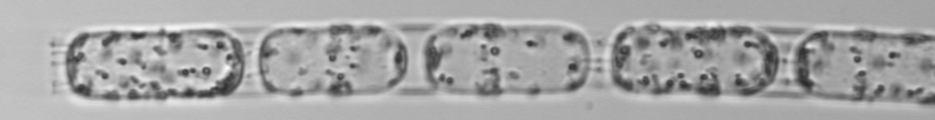
\includegraphics[width=10cm,height=2cm]{4.png}} 
  \hspace{0.3in} 
  \subfigure[log enhancement image]{ 
    \label{fig:subfig:b} %% label for second subfigure 
    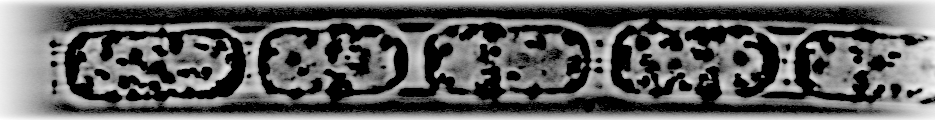
\includegraphics[width=10cm,height=2cm]{3.png}} 
   \hspace{0.3in} 
   \subfigure[histogram enhancement1]{ 
    \label{fig:subfig:b} %% label for second subfigure 
    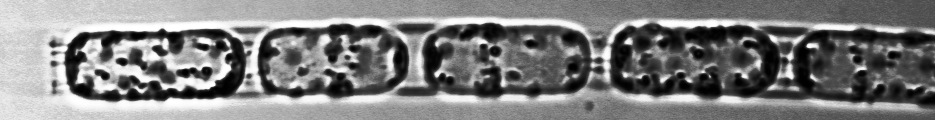
\includegraphics[width=10cm,height=2cm]{2.png}} 
   \hspace{0.3in} 
   \subfigure[histogram enhancement2]{ 
    \label{fig:subfig:b} %% label for second subfigure 
    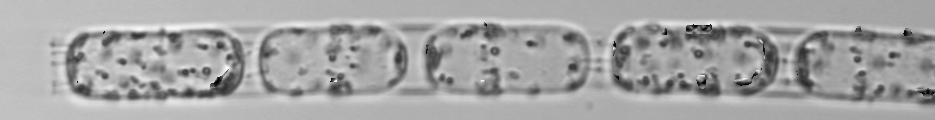
\includegraphics[width=10cm,height=2cm]{1.png}} 
   \hspace{0.3in} 
  \caption{Similar in shapes but different in textures} 
  \label{fig:subfig} %% label for entire figure 
\end{figure}



\section{Denoise}
\subsection{Experiment Objective}
Fig.2 shows that the image after enhancement will suffer great salt noise,  this week, I also try different median filtering methods to remove the salt noise. I used Geometric Mean Filter, Contrary Harmonic Mean Filter, Midpoint Filter and Median Filter(3*3). 

\begin{figure}[!ht]
\centering
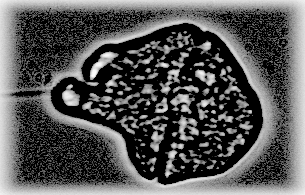
\includegraphics[width=10cm,height=7cm]{5.png}
\caption{image after enhancement}
\hspace{0.05in}
\label{fig: image after enhancement}
\end{figure}

\subsection{Experiment Result}

\begin{figure}[!ht] 
  \centering 
  \subfigure[midpoint filter]{ 
    \label{fig:subfig:a} %% label for first subfigure 
    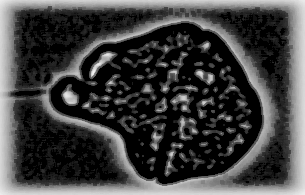
\includegraphics[width=6cm,height=4cm]{6.png}} 
  \hspace{0.3in} 
  \subfigure[median filter]{ 
    \label{fig:subfig:b} %% label for second subfigure 
    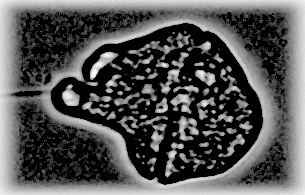
\includegraphics[width=6cm,height=4cm]{7.png}} 
   \hspace{0.3in} 
   \subfigure[Geometric filter]{ 
    \label{fig:subfig:b} %% label for second subfigure 
    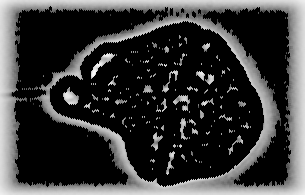
\includegraphics[width=6cm,height=4cm]{8.png}} 
   \hspace{0.3in} 
   \subfigure[Contrary Harmonic Mean Filter]{ 
    \label{fig:subfig:b} %% label for second subfigure 
    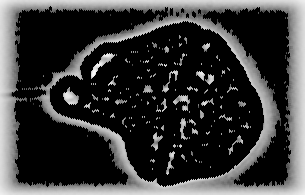
\includegraphics[width=6cm,height=4cm]{9.png}} 
   \hspace{0.3in} 
  \caption{Similar in shapes but different in textures} 
  \label{fig:subfig} %% label for entire figure 
\end{figure}

\subsection{Experiment Summary}
The result shows that result of median filtering is the best. But there is still some noise on the background, so I do two times or three times filtering, the result shows that, more filtering will lead to the details which we want to emphasize becoming blurred. From the third experiment and the forth experiment I think it difficult at least time-consuming to find a good method to do enhancement or filtering, because this kinds of methods will 'hurt' texture, we must 'protect' out texture to remove noises.


\begin{figure}[!ht]
\centering
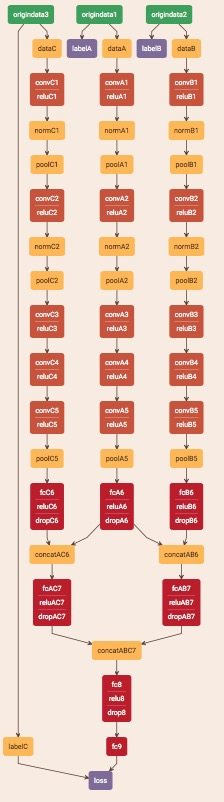
\includegraphics[width=8cm,height=23cm]{3.jpg}
\caption{Structure of our neural network.}
\hspace{0.05in}
\label{fig:network}
\end{figure}

\end{document}